\chapter{超音速牛奶喷射的概率动力学}

本章建立一个用于演示的超音速喷射参数模型。内容不对应真实实验结论，但覆盖物理记号、行内公式、行间公式、参数表和单位排版，便于将本章替换为真实研究内容时复用结构。

\section{超音速喷射模型}

\subsection{喷射过程与基本假设}

针对超音速牛奶喷射过程，示例模型将喷嘴出口速度、流体黏度和环境压力作为主要参数，并在稳态条件下讨论喷流的形成与传播。设喷嘴出口截面积为 $A_0$、特征长度为 $L$、流体密度为 $\rho$，则质量流率可以作为连接实验观测与动力学模型的中间量。实际论文中应给出装置、测量不确定度和边界条件，而不应只保留符号定义。

为了说明物理过程、几何关系和状态变量之间的差别，图~\ref{fig:ch2-schematics}将四种常见示意图放在同一组中：波动场、三角几何关系、场线与介质以及表达式树。示意图帮助读者理解变量关系，并不替代实验装置图或数值结果。
\begin{figure}[htbp]
  \centering
  \subfigure[叠加波动场]{
    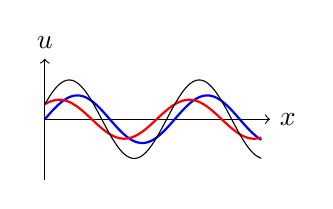
\begin{tikzpicture}[scale=0.55]
      \draw[->] (0,0)--(5.2,0) node[right] {$x$};
      \draw[->] (0,-1.4)--(0,1.4) node[above] {$u$};
      \draw[blue,domain=0:5,samples=80,smooth,thick] plot(\x,{0.55*sin(120*\x)});
      \draw[red,domain=0:5,samples=80,smooth,thick] plot(\x,{0.45*sin(120*\x+50)});
      \draw[black,domain=0:5,samples=80,smooth] plot(\x,{0.55*sin(120*\x)+0.45*sin(120*\x+50)});
    \end{tikzpicture}}
  \hfill
  \subfigure[几何关系与角度]{
    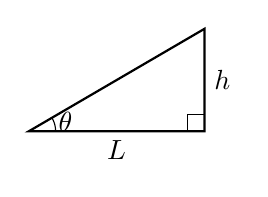
\begin{tikzpicture}[scale=0.62]
      \draw[thick] (0,0)--(3.6,0)--(3.6,2.1)--cycle;
      \draw (3.25,0)--(3.25,0.35)--(3.6,0.35);
      \draw (0.55,0) arc (0:30:0.55);
      \node at (0.75,0.19) {$\theta$};
      \node[below] at (1.8,0) {$L$};
      \node[right] at (3.6,1.05) {$h$};
    \end{tikzpicture}}
  \\
  \subfigure[场线与介质区域]{
    \begin{tikzpicture}[scale=0.62]
      \draw[thick] (0,0) rectangle (4.6,1.8);
      \fill[blue!8] (1.6,0.15) rectangle (3.1,1.65);
      \draw[thick] (1.6,0.15) rectangle (3.1,1.65);
      \foreach \y in {0.35,0.65,0.95,1.25,1.55}
        \draw[-{Stealth},blue] (0.25,\y)--(4.25,\y);
      \node at (2.35,0.9) {介质};
    \end{tikzpicture}}
  \hfill
  \subfigure[表达式树结构]{
    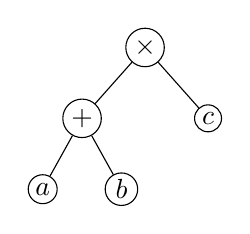
\begin{tikzpicture}[level distance=9mm,sibling distance=16mm,
      every node/.style={draw,circle,inner sep=1.3pt},
      level 2/.style={sibling distance=10mm}]
      \node {$\times$}
        child {node {$+$}
          child {node {$a$}}
          child {node {$b$}}}
        child {node {$c$}};
    \end{tikzpicture}}
  \caption{建模视角示意图组：连续场、几何约束、介质区域与离散结构}
  \label{fig:ch2-schematics}
\end{figure}

这些图形分别对应连续场、几何约束、介质区域和离散结构四种建模视角。真实论文中应为每张图配套说明变量、边界条件和数据来源，而不是把绘图工具本身作为结果。

在连续介质近似下，速度场 $\bm{v}$ 的旋度和梯度可以使用统一的向量记号表达：
\begin{equation}
  \nabla\times\nabla\phi=\bm{0},\qquad
  T^{\mu\nu}=T_{\mu}^{\ \nu},\qquad
  \frac{\partial^2p}{\partial x\,\partial y}.
  \label{eq:physica-notation}
\end{equation}
式~\eqref{eq:physica-notation}只展示记号形式；实际研究中应根据张量的坐标变换规则和物理量的量纲给出完整推导。

当示意图需要同时表达结构关系和数学标注时，图~\ref{fig:state-space-diagram}展示观测量、状态更新和参数后验之间的联系。预测结果返回下一轮观测，图内公式与本章状态更新记号一致，便于与正文公式对照。
\begin{figure}[htbp]
  \centering
  \begin{tikzpicture}[
    node distance=13mm and 16mm,
    box/.style={draw,rounded corners=2pt,minimum width=34mm,minimum height=12mm,align=center,line width=.55pt,font=\small},
    arrow/.style={-{Stealth[length=2.1mm]},line width=.6pt}
  ]
    \node[box,fill=gray!6] (obs) {观测量\\$\bm{y}_k$};
    \node[box,fill=gray!6,right=of obs] (state) {状态更新\\$\bm{x}_{k+1}=A\bm{x}_k+\bm{w}_k$};
    \node[box,fill=gray!6,right=of state] (post) {参数后验\\$p(\theta\mid\bm{y}_{1:k})$};
    \draw[arrow] (obs)--node[above,font=\scriptsize] {$H\bm{x}_k+\bm{v}_k$}(state);
    \draw[arrow] (state)--node[above,font=\scriptsize] {贝叶斯更新}(post);
    \draw[arrow] (post.south)--++(0,-10mm)-|node[pos=.48,below,font=\scriptsize] {预测}(obs.south);
  \end{tikzpicture}
  \caption{统一字体的状态空间示意图}
  \label{fig:state-space-diagram}
\end{figure}

\subsection{概率分布与实验指标}

在参数分析中，可以用概率分布描述喷射速度和喷射效率的离散性。设出口速度观测值为 $v_i$，样本均值和样本方差分别为 $\bar{v}$ 与 $s_v^2$，则重复实验可以用置信区间报告，而不应只报告一个看似精确的平均值。真实论文应给出实验装置、数据来源、计算方法及其误差分析。

当前示例使用模板本地字体和显式单位文本，避免把存在兼容性问题的 Metro 宏包带入默认论文构建。LaTeX 版本可用 `siunitx` 把数值与单位绑定书写：例如出口速度写成 $340~\mathrm{m\,s^{-1}}$，测量误差写成 $(340\pm5)~\mathrm{m\,s^{-1}}$，有效工作区间写成 $0.20$--$0.80~\mathrm{mm}$。这样单位、数字和误差不会因为手工空格不同而在各章节中产生不一致的视觉结果。

在真实论文中，实验量应始终与单位绑定。例如，喷嘴出口速度、测量误差和有效工作区间可以分别用 `\qty{340}{\meter\per\second}`、`\qty{340 \pm 5}{\meter\per\second}` 和 `\qtyrange{0.20}{0.80}{\milli\meter}` 表示。应先确认所用单位宏包的版本与模板兼容，再将同一接口用于全文。

为了避免只展示平均值，本章再给出一组小型数据诊断图。折线图带有误差线，散点图用颜色表达第三个量，柱状图适合汇总离散指标，箱线图则用于比较重复实验的分布。图~\ref{fig:ch2-diagnostics}中的数据是排版示例，正式论文中应替换为真实观测值，并在正文中解释误差来源。
\begin{figure}[htbp]
  \centering
  \subfigure[误差线折线图]{
    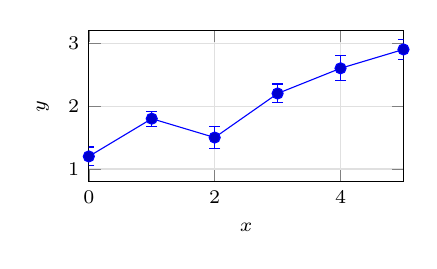
\begin{tikzpicture}
      \begin{axis}[width=.46\textwidth,height=3.5cm,xmin=0,xmax=5,ymin=0.8,ymax=3.2,
        xlabel={$x$},ylabel={$y$},tick label style={font=\scriptsize},
        label style={font=\scriptsize},grid=major,grid style={black!12}]
        \addplot+[blue,mark=*,error bars/.cd,y dir=both,y explicit]
          coordinates {(0,1.2) +- (0,0.15) (1,1.8) +- (0,0.12) (2,1.5) +- (0,0.18)
                       (3,2.2) +- (0,0.15) (4,2.6) +- (0,0.20) (5,2.9) +- (0,0.16)};
      \end{axis}
    \end{tikzpicture}}
  \hfill
  \subfigure[彩色散点图]{
    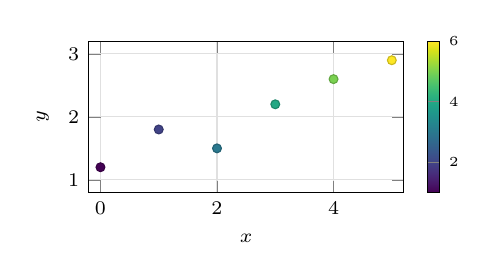
\begin{tikzpicture}
      \begin{axis}[width=.46\textwidth,height=3.5cm,xmin=-.2,xmax=5.2,ymin=.8,ymax=3.2,
        xlabel={$x$},ylabel={$y$},tick label style={font=\scriptsize},
        label style={font=\scriptsize},grid=major,grid style={black!12},
        colormap/viridis,colorbar,colorbar style={width=1.5mm,tick label style={font=\tiny}}]
        \addplot[only marks,scatter,point meta=explicit,mark=*,mark size=1.6pt]
          table[meta=c,row sep=crcr] {
            x y c\\
            0 1.2 1\\
            1 1.8 2\\
            2 1.5 3\\
            3 2.2 4\\
            4 2.6 5\\
            5 2.9 6\\
          };
      \end{axis}
    \end{tikzpicture}}
  \\
  \subfigure[指标柱状图]{
    \begin{tikzpicture}
      \begin{axis}[width=.46\textwidth,height=3.5cm,ymin=0,ymax=3.0,
        ybar,bar width=8pt,symbolic x coords={1,2,3,4},xtick=data,
        xlabel={指标},ylabel={数值},tick label style={font=\scriptsize},
        label style={font=\scriptsize},grid=major,grid style={black!12},
        nodes near coords, nodes near coords style={font=\tiny}]
        \addplot[fill=teal!55,draw=teal!70!black] coordinates {(1,1.3) (2,2.1) (3,1.7) (4,2.6)};
      \end{axis}
    \end{tikzpicture}}
  \hfill
  \subfigure[重复实验分布]{
    \begin{tikzpicture}
      \begin{axis}[width=.46\textwidth,height=3.5cm,ymin=.8,ymax=3.2,
        boxplot/draw direction=y,xtick={1,2,3},xticklabels={A,B,C},
        xlabel={重复实验组},ylabel={观测值},tick label style={font=\scriptsize},
        label style={font=\scriptsize},grid=major,grid style={black!12}]
        \addplot+[boxplot prepared={lower whisker=1.0,lower quartile=1.3,median=1.6,upper quartile=2.2,upper whisker=2.8},fill=blue!15] coordinates {};
        \addplot+[boxplot prepared={lower whisker=1.4,lower quartile=1.8,median=2.1,upper quartile=2.55,upper whisker=3.0},fill=teal!15] coordinates {};
        \addplot+[boxplot prepared={lower whisker=1.1,lower quartile=1.65,median=2.0,upper quartile=2.35,upper whisker=2.9},fill=orange!18] coordinates {};
      \end{axis}
    \end{tikzpicture}}
  \caption{重复实验数据的诊断图组}
  \label{fig:ch2-diagnostics}
\end{figure}

\subsection{公式、参数与三线表示例}

正文中的行内公式可以直接写在段落中，例如马赫数 $\mathrm{Ma}=v/a$ 和雷诺数 $\mathrm{Re}=\rho vL/\mu$。较长的推导使用带编号的行间公式，以便在后文通过交叉引用定位。
\begin{equation}
  \mathrm{Re}=\frac{\rho vL}{\mu},\qquad \mathrm{Ma}=\frac{v}{a}.
  \label{eq:dimensionless-numbers}
\end{equation}

需要对齐多行等式时，可使用 \texttt{align} 环境；换行后的各行可以共享同一个公式编号。偏导数的混合阶数也可以直接写进公式，从而让复杂模型的推导结构保持可读：
\begin{equation}
  \begin{aligned}
    m &= \rho V,\\
    q &= mc_p(T_2-T_1),\\
    \eta &= \frac{q}{q_{\mathrm{in}}}.
  \end{aligned}
  \label{eq:aligned-example}
\end{equation}
\begin{equation}
  \frac{\partial^2p}{\partial x\,\partial y}
  =\frac{\partial}{\partial x}\left(\frac{\partial p}{\partial y}\right).
  \label{eq:mixed-derivative}
\end{equation}

表~\ref{tab:parameters}展示参数、符号和示例值的常见组织方式。正式论文中可把示例值替换为实验数据，并在表格外补充数据来源和单位说明。
\begin{table}[htbp]
  \centering
  \caption{三线表示例：模型参数}
  \label{tab:parameters}
  \begin{tabular}{cccc}
    \toprule
    \textbf{参数} & \textbf{符号} & \textbf{示例取值} & \textbf{单位}\\
    \midrule
    喷嘴出口速度 & $v_0$ & $340$ & \si{\meter\per\second}\\
    特征长度 & $L$ & $0.012$ & \si{\meter}\\
    动力黏度 & $\mu$ & $1.8$ & \si{\milli\pascal\second}\\
    出口压力 & $p_0$ & $1.01\times10^5$ & \si{\pascal}\\
    \bottomrule
  \end{tabular}

  \smallskip
  \begin{minipage}{0.88\textwidth}\footnotesize
    注：表中为示例取值，正式论文应给出数据来源、测量方法与不确定度。
  \end{minipage}
\end{table}

公式标签示例见式~\eqref{eq:dimensionless-numbers}。公式内容或章节顺序变化时，编号和引用会自动更新。

\section{数学工具与表示}

\subsection{张量、矩阵与范数}

模型中的参数、观测和中间量分别用标量、向量和张量表示。写成矩阵形式后，状态转移、参数辨识和误差传播可以共用同一套记号，不必在正文里反复展开分量求和。下面的写法同时给出紧凑形式和按分量展开的形式，便于读者在两种表达之间切换。
\begin{equation}
  \bm{A}=
  \begin{bmatrix}
    a_{11}&a_{12}&\cdots&a_{1n}\\
    a_{21}&a_{22}&\cdots&a_{2n}\\
    \vdots&\vdots&\ddots&\vdots\\
    a_{m1}&a_{m2}&\cdots&a_{mn}
  \end{bmatrix},
  \qquad
  \bm{x}=
  \begin{bmatrix}x_1&x_2&\cdots&x_n\end{bmatrix}^{\mathsf T}.
  \label{eq:matrix-vector}
\end{equation}

矩阵与向量的乘积、二次型和行列式是后续推导中出现频率最高的三种运算。二次型用于表示能量和代价，行列式用于判断线性变换是否可逆，也出现在变量替换的雅可比因子中。
\begin{equation}
  (\bm{A}\bm{x})_i=\sum_{j=1}^{n}a_{ij}x_j,\quad
  \bm{x}^{\mathsf T}\bm{A}\bm{x}
    =\sum_{i=1}^{n}\sum_{j=1}^{n}a_{ij}x_ix_j,\quad
  \det(\bm{A})=\sum_{\sigma\in S_n}\operatorname{sgn}(\sigma)
    \prod_{i=1}^{n}a_{i,\sigma(i)}.
  \label{eq:matrix-ops}
\end{equation}

度量向量和矩阵的大小需要范数：二范数用来描述观测残差，Frobenius 范数用来描述参数矩阵的整体偏离，谱范数则给出最坏方向上的放大倍数。真实论文应说明各符号的维度、量纲和取值区间，而不应只给出矩阵形状。
\begin{equation}
  \|\bm{x}\|_2=\sqrt{\sum_{i=1}^{n}x_i^2},\qquad
  \|\bm{A}\|_{\mathrm F}=\sqrt{\operatorname{tr}(\bm{A}^{\mathsf T}\bm{A})},\qquad
  \|\bm{A}\|_2=\max_{\|\bm{x}\|_2=1}\|\bm{A}\bm{x}\|_2.
  \label{eq:norms}
\end{equation}

\subsection{级数、积分与极限}

把连续过程离散化时，时间步长和截断阶数决定了需要保留多少项。等比级数给出误差项的上界，连乘形式适合描述逐步累积的衰减，含参积分则用于把边界条件并入解的表达式中。
\begin{equation}
  \sum_{k=0}^{\infty}q^k=\frac{1}{1-q},\quad |q|<1;\qquad
  \sum_{k=1}^{n}k=\frac{n(n+1)}{2};\qquad
  \prod_{i=1}^{n}(1-\varepsilon_i)\approx1-\sum_{i=1}^{n}\varepsilon_i.
  \label{eq:series}
\end{equation}

当被积函数含有指数衰减或振荡因子时，解析结果往往可以写成初等函数的组合。下式给出两类在响应分析中反复出现的积分，它们的量纲分别对应时间尺度和幅值密度。
\begin{equation}
  \int_{0}^{\infty}e^{-\lambda t}\,\mathrm{d}t=\frac{1}{\lambda},\qquad
  \int_{-\infty}^{\infty}e^{-ax^2+bx}\,\mathrm{d}x
    =\sqrt{\frac{\pi}{a}}e^{b^2/(4a)},\quad a>0.
  \label{eq:integrals}
\end{equation}

极限记号用于说明离散格式的收敛性。若步长趋于零时截断误差以二阶速度下降，则加密网格带来的收益是可以预期的。
\begin{equation}
  \lim_{n\to\infty}\left(1+\frac{1}{n}\right)^n=e,\qquad
  \lim_{h\to0}\frac{f(x+h)-2f(x)+f(x-h)}{h^2}=f''(x).
  \label{eq:limits}
\end{equation}

\subsection{微分算子与场论}

喷射流场既可以用分量形式写出，也可以用算符形式写出。算符形式的优点是物理含义清晰：梯度给出最快的增长方向，散度衡量源的强度，旋度描述局部旋转，而拉普拉斯算子把扩散与源项联系在同一方程中。
\begin{equation}
  \nabla\phi=
  \left(\frac{\partial\phi}{\partial x},
  \frac{\partial\phi}{\partial y},
  \frac{\partial\phi}{\partial z}\right),\qquad
  \nabla\cdot\bm{v}=
  \frac{\partial v_x}{\partial x}
  +\frac{\partial v_y}{\partial y}
  +\frac{\partial v_z}{\partial z}.
  \label{eq:field-operators}
\end{equation}

旋度写成行列式形式更紧凑，也便于检查分量中偏导数的配对关系：
\begin{equation}
  \nabla\times\bm{v}=
  \begin{vmatrix}
    \bm{e}_x&\bm{e}_y&\bm{e}_z\\
    \partial_x&\partial_y&\partial_z\\
    v_x&v_y&v_z
  \end{vmatrix}
  =
  \left(
  \frac{\partial v_z}{\partial y}-\frac{\partial v_y}{\partial z},
  \frac{\partial v_x}{\partial z}-\frac{\partial v_z}{\partial x},
  \frac{\partial v_y}{\partial x}-\frac{\partial v_x}{\partial y}
  \right).
  \label{eq:curl}
\end{equation}

把算符组合起来可以得到守恒律和输运方程。下面的对流扩散方程在示例模型里用于描述速度场与浓度场之间的耦合，方程中的每一项都应对应正文中说明过的物理机制。
\begin{equation}
  \frac{\partial c}{\partial t}+\bm{v}\cdot\nabla c
    =D\nabla^2c+s(\bm{x},t),\qquad
  \frac{\partial\bm{v}}{\partial t}
    +(\bm{v}\cdot\nabla)\bm{v}
    =-\frac{1}{\rho}\nabla p+\nu\nabla^2\bm{v}.
  \label{eq:transport}
\end{equation}

\subsection{概率分布与贝叶斯更新}

观测的离散性用概率分布描述。正态密度适合连续量，指数分布适合等待时间，多项分布适合计数；三者的参数都应给出估计方法和置信区间，而不应只给一个点值。
\begin{equation}
  p(x)=\frac{1}{\sigma\sqrt{2\pi}}
    \exp\!\left[-\frac{(x-\mu)^2}{2\sigma^2}\right],\qquad
  p(t)=\lambda e^{-\lambda t},\qquad
  P(\bm{n})=\frac{N!}{\prod_i n_i!}\prod_i p_i^{n_i}.
  \label{eq:distributions}
\end{equation}

期望和方差是分布的两个基本数字特征。样本量较小时应以区间形式报告结果，因为均值的标准误随样本量按平方根下降，单次实验的波动往往大于均值本身。
\begin{equation}
  \begin{aligned}
    \mathbb{E}[X] &=
      \int_{-\infty}^{\infty}xp(x)\,\mathrm{d}x,\\
    \operatorname{Var}[X] &=
      \mathbb{E}\!\left[(X-\mathbb{E}[X])^2\right]
      =\mathbb{E}[X^2]-\mathbb{E}[X]^2,\\
    \operatorname{se}(\bar{X}) &= \frac{\sigma}{\sqrt{n}}.
  \end{aligned}
  \label{eq:moments}
\end{equation}

参数更新写成贝叶斯形式后，先验、似然和后验的关系一目了然。分母是与参数无关的归一化常数，因此工程上常写成正比形式，把计算量集中在似然函数的求值上。
\begin{equation}
  p(\theta\mid\bm{y})=
  \frac{p(\bm{y}\mid\theta)p(\theta)}
  {\int p(\bm{y}\mid\theta')p(\theta')\,\mathrm{d}\theta'},\qquad
  p(\theta\mid\bm{y})\propto p(\bm{y}\mid\theta)p(\theta).
  \label{eq:bayes}
\end{equation}

两个独立随机变量之和的分布由卷积给出。卷积还可以用来描述测量系统的响应：观测序列等于真实信号与仪器冲激响应的卷积再加上噪声。
\begin{equation}
  (f*g)(t)=\int_{-\infty}^{\infty}f(\tau)g(t-\tau)\,\mathrm{d}\tau,\qquad
  y(t)=(h*u)(t)+\varepsilon(t).
  \label{eq:convolution}
\end{equation}

把信号从时域变换到频域后，卷积变成乘积，滤波和谱分析可以在同一个框架下处理。变换对的存在性条件和采样定理应在正文中说明，避免把离散频谱直接当成连续谱使用。
\begin{equation}
  F(\omega)=\int_{-\infty}^{\infty}f(t)e^{-\mathrm{i}\omega t}\,\mathrm{d}t,\qquad
  f(t)=\frac{1}{2\pi}\int_{-\infty}^{\infty}
  F(\omega)e^{\mathrm{i}\omega t}\,\mathrm{d}\omega,\qquad
  f_s>2f_{\max}.
  \label{eq:fourier}
\end{equation}

\subsection{样例计算公式}

下面的分段函数用于说明条件判断在公式中的写法：不同工况对应不同的衰减规律，开关量则由区间条件给出。
\begin{equation}
  \eta(v)=
  \begin{cases}
    1-v/v_0, & v\leq v_0,\\
    (v_0/v)^2, & v_0<v\leq2v_0,\\
    0, & v>2v_0.
  \end{cases}
  \label{eq:piecewise}
\end{equation}

统计指标把一组观测压缩成一个数，报出时必须同时给出样本量和区间。下式给出常用的误差与拟合优度定义，用于第 4 章的模拟结果比较。
\begin{equation}
  \mathrm{RMSE}=\sqrt{\frac{1}{n}\sum_{i=1}^{n}(y_i-\hat{y}_i)^2},\qquad
  \mathrm{MAE}=\frac{1}{n}\sum_{i=1}^{n}|y_i-\hat{y}_i|,\qquad
  R^2=1-\frac{\sum_i(y_i-\hat{y}_i)^2}{\sum_i(y_i-\bar{y})^2}.
  \label{eq:error-metrics}
\end{equation}

\section{公式版式与编号}

本节把模板支持的公式版式集中列出，便于按内容选择：行内与行间、多行对齐、逐行编号、分段函数、矩阵与方程组、大算符、连分数、上下标注、集合与映射、指标式、概率记号、变换对、泛函、数值与单位。每种版式都给出适用条件，正式论文按同样的规则书写即可保持编号与间距一致。

\subsection{行内公式与行间公式}

行内公式跟随文字基线，适合短表达式：能量换算 $E=mc^2$、无量纲数 $\mathrm{Ma}=v/a$、集合关系 $x\in\mathcal{X}$。较长的式子独立成行并自动编号，正文用标签引用：
\begin{equation}
  \int_0^L \rho A(x)\dot{x}^{\,2}\,\mathrm{d}x=2E_k.
  \label{eq:kinetic-energy-integral}
\end{equation}

\subsection{多行对齐与逐行编号}

多行推导用 \texttt{align} 环境指定对齐点并换行，整块共享一个公式编号；需要逐行编号时把每行写成独立公式，编号会连续给出：
\begin{equation}
  \begin{aligned}
    m &= \rho V,\\
    q &= mc_p(T_2-T_1),\\
    \eta &= q/q_{\mathrm{in}}.
  \end{aligned}
  \label{eq:aligned-derivation}
\end{equation}
\begin{equation}P_1V_1=nRT_1.\label{eq:state-1}\end{equation}
\begin{equation}P_2V_2=nRT_2.\label{eq:state-2}\end{equation}

\subsection{分段函数与条件}

分段定义用 \texttt{cases} 环境：左花括号由环境给出，条件列按对齐点排列。若分段表达式中包含较长的分式，可使用 \texttt{\textbackslash displaystyle} 维持可读字号：
\begin{equation}
  C_D(\bm{v})=
  \begin{cases}
    C_0, & \|\bm{v}\|\leq v_c,\\
    C_0\left(v_c/\|\bm{v}\|\right)^2, & \|\bm{v}\|>v_c.
  \end{cases}
  \label{eq:piecewise-drag}
\end{equation}

\subsection{矩阵、向量与方程组}

矩阵用 \texttt{bmatrix}、\texttt{pmatrix} 等环境表示；分块矩阵按行列书写，带竖线的矩阵用于表示行列式或范数。需要在正文中保持维数关系时，应把矩阵的阶数写在正文而不是塞进公式：
\begin{equation}
  \bm{A}=
  \begin{pmatrix}1&2&0\\0&1&-1\\2&0&1\end{pmatrix},\qquad
  \det(\bm{A})=
  \begin{vmatrix}1&2&0\\0&1&-1\\2&0&1\end{vmatrix},\qquad
  \bm{M}=
  \begin{bmatrix}\bm{A}&\bm{B}\\\bm{C}&\bm{0}\end{bmatrix}.
  \label{eq:matrix-family}
\end{equation}

方程组用 \texttt{cases} 与对齐点表示；带条件的约束放在第二列，条件相同的一组方程共用一个编号：
\begin{equation}
  \begin{cases}
    \dot{\bm{x}}=\bm{A}\bm{x}+\bm{B}\bm{u}, & t>0,\\
    \bm{y}=\bm{C}\bm{x}, & t\geq0.
  \end{cases}
  \label{eq:system}
\end{equation}

\subsection{大算符、极限与最值}

求和、连乘、积分、极限与最值都支持上下限；显示模式下上下限排在算符的上方和下方，行内模式下自动改为右侧上下标：
\begin{equation}
  \sum_{i=1}^{n}w_ix_i,\qquad
  \prod_{k=1}^{m}(1+r_k),\qquad
  \int_{\Omega}f(\bm{x})\,\mathrm{d}\bm{x}.
  \label{eq:big-operators}
\end{equation}
\begin{equation}
  \lim_{n\to\infty}a_n,\qquad
  \max_{\bm{x}\in\mathcal{X}}f(\bm{x}),\qquad
  \operatorname*{arg\,min}_{\bm{\theta}}L(\bm{\theta}).
  \label{eq:limits-extrema}
\end{equation}

\subsection{连分数与嵌套结构}

连分数与嵌套根式写成斜线形式时层级较多，再逐层恢复全尺寸会撑高公式；层数较多时应改用递推式表示，并在正文说明截断项数：
\begin{equation}
  \sqrt{2}=1+\frac{1}{2+\frac{1}{2+\frac{1}{2+\cdots}}},\qquad
  \phi=1+\frac{1}{1+\frac{1}{1+\frac{1}{1+\cdots}}}.
  \label{eq:continued-fraction}
\end{equation}

\subsection{上下标注}

把推导中的每一项直接标注出来，比在图注里解释更直观：
\begin{equation}
  \underbrace{\|\hat{\bm{y}}-\bm{y}\|}_{\text{残差}}
  =\underbrace{C_1h^p}_{\text{格式误差}}
  +\underbrace{C_2\delta}_{\text{数据误差}}.
  \label{eq:annotated-sum}
\end{equation}

\subsection{集合、映射与逻辑}

集合与映射的记号用于定义变量的取值范围；量词与箭头用于描述连续性和收敛性。写极限定义时应同时给出邻域半径与误差限：
\begin{equation}
  f:\mathcal{X}\to\mathcal{Y},\quad x\mapsto f(x),\quad
  \mathcal{A}\subseteq\mathcal{X},\quad
  \mathcal{A}\cup\mathcal{B},\quad
  \mathcal{A}\cap\mathcal{B},\quad x\notin\mathcal{A}.
  \label{eq:set-mapping}
\end{equation}
\begin{equation}
  \forall\varepsilon>0,\ \exists\delta>0:
  \|\bm{x}-\bm{x}_0\|<\delta
  \Rightarrow
  \|f(\bm{x})-f(\bm{x}_0)\|<\varepsilon.
  \label{eq:continuity}
\end{equation}

\subsection{张量与指标式}

张量用上下标表示指标，重复指标按求和约定处理；矩阵乘法写成指标式后，维数是否匹配可以直接看出：
\begin{equation}
  T^{\mu\nu}=\eta^{\mu\alpha}\eta^{\nu\beta}T_{\alpha\beta},\qquad
  (\bm{A}\bm{B})_{ij}=\sum_{k=1}^{n}a_{ik}b_{kj},\qquad
  \partial_\alpha F^{\alpha\beta}=\mu_0J^\beta.
  \label{eq:tensor-index}
\end{equation}

\subsection{概率与期望记号}

概率与期望的记号集中在这里定义，避免同一含义在不同章节写法不一致。指示函数用带下标的 $\mathbf{1}$，取值只有 0 和 1 两种：
\begin{equation}
  \begin{aligned}
    \mathbb{E}[X]&=\int_{-\infty}^{\infty}xp_X(x)\,\mathrm{d}x,\\
    \operatorname{Cov}[X,Y]&=\mathbb{E}[(X-\mu_X)(Y-\mu_Y)],\\
    \mathbf{1}_{A}(\omega)&=
    \begin{cases}
      1,&\omega\in A,\\
      0,&\omega\notin A.
    \end{cases}
  \end{aligned}
  \label{eq:probability-notation}
\end{equation}

\subsection{变换对与泛函}

变换对用两行对齐写出正变换与逆变换，等号对齐后读者容易核对系数；泛函的极值条件由 Euler--Lagrange 方程给出，导数的阶数决定边界条件的个数：
\begin{equation}
  \begin{aligned}
    F(\omega)&=\int_{-\infty}^{\infty}f(t)e^{-\mathrm{i}\omega t}\,\mathrm{d}t,\\
    f(t)&=\frac{1}{2\pi}\int_{-\infty}^{\infty}
      F(\omega)e^{\mathrm{i}\omega t}\,\mathrm{d}\omega.
  \end{aligned}
  \label{eq:transform-pair}
\end{equation}
\begin{equation}
  \frac{\partial L}{\partial y}
  -\frac{\mathrm{d}}{\mathrm{d}x}
  \left(\frac{\partial L}{\partial y'}\right)=0.
  \label{eq:euler-lagrange}
\end{equation}

\subsection{数值与单位}

带单位和误差的数值应采用统一写法，使单位、数字和误差各自占据固定位置，不会因手工空格不同而在各章产生不一致：喷嘴出口速度 $340~\mathrm{m\,s^{-1}}$，测量误差 $(340\pm5)~\mathrm{m\,s^{-1}}$，有效工作区间 $0.20$--$0.80~\mathrm{mm}$。

\subsection{公式编号与引用}

公式编号按章编排（如式~\eqref{eq:aligned-derivation}、式~\eqref{eq:tensor-index}），标签不变时插入新公式只会影响后续编号，引用处会自动更新。正文引用应写“由式~\eqref{eq:taylor}可得”，不要写“由上式可得”，否则插入新公式后指代会整体错位。

\section{本章小结}

本章示例建立了从物理假设到指标分析的基本结构，为后续章节的模型验证提供接口。
